\section{Jadrá korekcie}

Ak medzi dvomi čítaniami nájdeme viacero jadier zarovnania, pravdepodobnosť, že čítania pochádzajú s prekrývajúcich sa úsekov genómu, je vysoká. Navyše od týchto jadier vyžadujeme, aby rozdiel pozícií v rámci čítania bol rovnaký, inak povedané ak $a_{1}$ a $a_{2}$ sú pozície prvého jadra na čítaniach a $b_{1}$ a $b_{2}$ sú pozície druhého jadra, potom $b_{1} - a_{1} \approx b_{2} - a_{2}$.

\begin{figure}
    \centering
    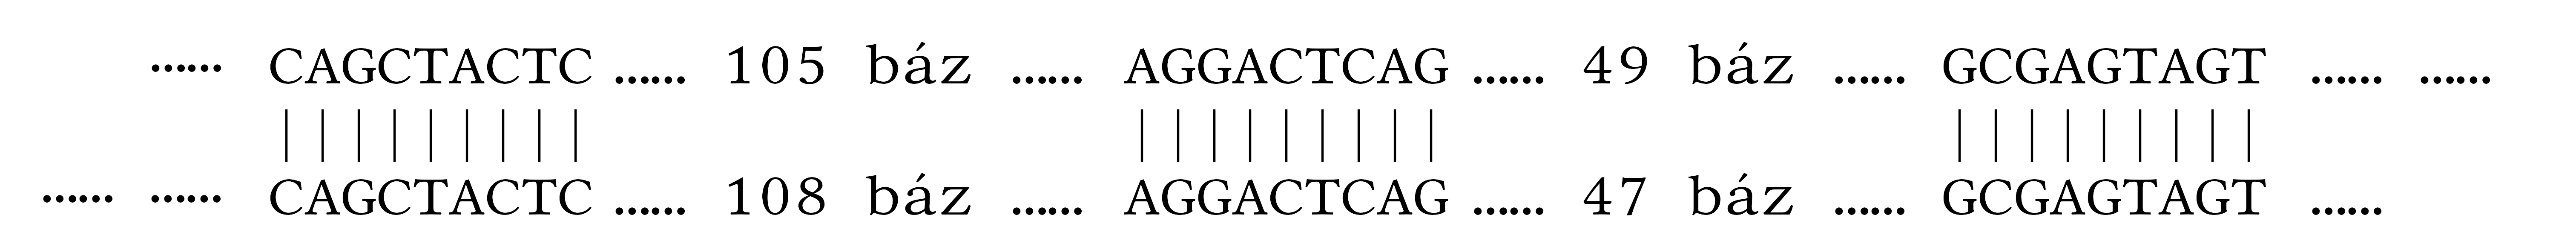
\includegraphics[width=1\textwidth]{images/jadra_korekcie.png}
    \caption{Viacero jadier medzi dvomi čítaniami}
    \label{fig:jadra_korekcie}
\end{figure} 

Aby bola v takomto jadre chyba, muselo by sekvenačné zariadenie urobiť na obidvoch čítaniach na tom istom mieste chybu rovnakého typu. V prípade substitúcie a inzercie by muselo  pridať resp. zameniť bázu za tú istú bázu. Tento fakt dáva jadrám vysokú mieru správnosti. Preto ich budeme používať ako základný stavebný prvok pri korekcii čítaní -- nazveme ich jadrá korekcie. 
Jadrá korekcie majú veľmi podobnú úlohu ako mali $k$-tice čítaní s nízkou chybovosťou v nástroji LoRDEC. $k$-tice vznikali zo súvislých sekvencií a susedné $k$-tice sa prekrývali na $k - 1$ znakoch, čo umožňovalo vytvoriť de Bruijnov graf. V našom prípade sú jadrá rozmiestnené náhodne a nemusí platiť, že na každej pozícii v genóme začína nejaké jadro zarovnania. Bude nutné použiť mierne odlyšné metódy.

\subsection{Hľadanie jadier}

Najprv sa však pozrieme ako v množine čítaní nájdeme jadrá korekcie. Našou úlohou je navrhnúť algoritmus, ktorý nájde všetky rovnaké súvislé podpostupnosti medzi všetkými dvojicami čítaní a následne vyberie tie dvojice čítaní, medzi ktorými je jadier zarovnania s priblížne rovnakými rozostupmi dostatočne veľa. Na samotné jadrá zarovnania existuje viacero algoritmov, niekoľko je dokonca uvedených v predchádzajúcej kapitole.

Ukázalo sa, že pri chybovosti čítaní sekvenačného zariadenia PacBio RS II je vhodná minimálna dĺžka jadier približne 13 báz. Ich dĺžka sa vyberá tak, aby jadier bolo dostatočne veľa, ale zároveň aby nevznikalo príliš veľa náhodných zhôd. Využijeme, že počet všetkých možných jadier pri danej dĺžke je $4^{13} = 67108864$. Jedna možnosť by bola vytvoriť polia pre každé možné jadro a tie by sa jedným prechodom cez všetky čítania naplnili. Tento prístup by ale spotreboval príliš veľa pamäte na alokácie, ktoré by sme museli urobiť aj pre $k$-tice vystkytujúce sa v čítaniach len raz. Namiesto toho algoritmus prechádza cez všetky čítania dvakrát. Pri prvom prechode len počíta výskyty rovnakých jadier. Používa na to pole veľkosti $4^{13}$ a indexuje sa sekvenciou kódovanou ako celé číslo. Kóduje sa tak, že jedna báza je reprezentovaná dvoma bitmi. Vypočíta prefixové sumy, ktoré potom slúžia ako indexy do jedného poľa so všetkými jadrami. Druhý prechod cez všetky čítania vyplní toto pole jadrami. Aby sme objavili zhody medzi čítaniami s opačnou orientáciou, zohľadníme pri oboch prechodoch aj pôvodné $k$-tice z čítania aj ich obrátené komplementárne sekvencie. Pre každú $k$-ticu si vo veľkom poli ukladáme identifikátor čítania, z ktorého pochádza, pozíciu vramci neho a či je to originálna, alebo obrátená sekvencia. 

\begin{figure}
    \centering
    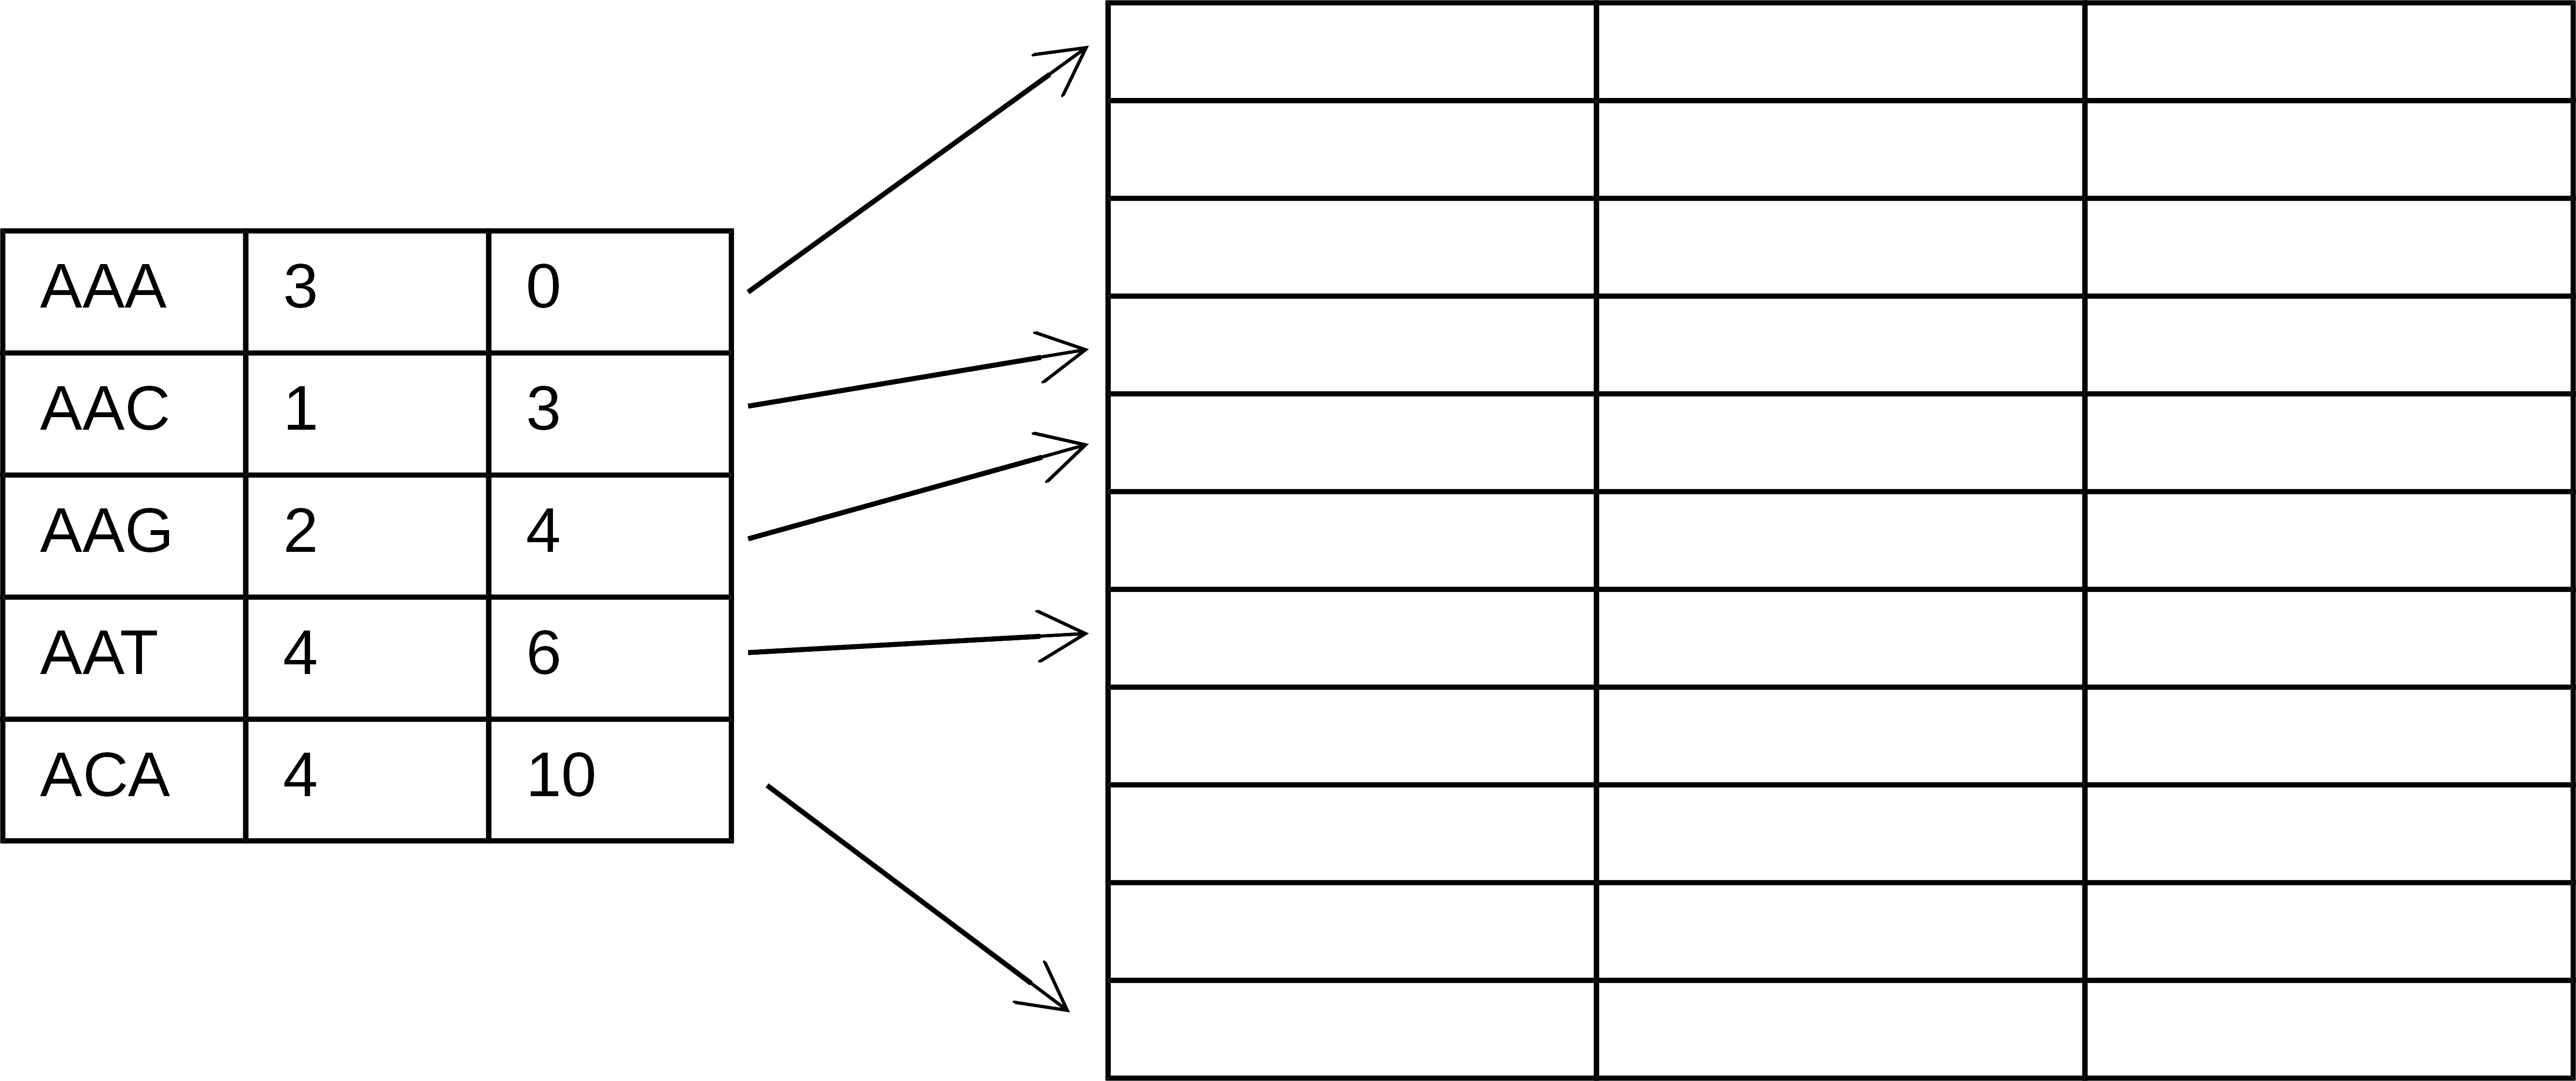
\includegraphics[width=1\textwidth]{images/jadra_velke_pole.png}
    \caption{Ukladanie jadier do jedného poľa}
    \label{fig:velke_pole}
\end{figure} 

\paragraph{Rozširovanie jadier}

Častokrát je súvislá zhoda medzi čítaniami na nejakom miste dlhšia ako $k$. Vtedy popísaný algoritmus nájde niekoľko po sebe idúcich, na $k - 1$ znakoch sa prekrývajúcich zhôd. Pre ďalšie spracovanie je výhodné spracovať tieto zhody ako jedno dlhšie jadro. Dosiahne sa to usporiadaním postupne podľa antidiagonály (rozdiel pozícií v čítaniach) a podľa pozície v niektorom z čítaní. Nadväzujúce jadrá sú po usporiadaní bezprostredne za sebou, čo umožní jednoduché spracovanie.

\paragraph{Detekcia prekrývajúcich sa čítaní}

